\chapter{Perception and Sensing in Robotics: Sensors and Algorithms}\label{ch:perceptionandsensing}
In this chapter we will discuss about robot perception in industrial settings, focusing the attention on the tools, e.g. sensors and software, and the techniques used to solve common industrial problems such as Random Bin Picking (RBP) and Pick\&Place (PPT). We will also introduce some state of the art commercial libraries that nowadays are commonly used in several industrial applications.

\section{Robotics in Industry}\label{sec:roboticsinindustry}
Over the years, industry has become one of the most important scenario where robots and automated systems have gained a widespread diffusion. This is basically thanks to the fact that robots can easily and quickly perform repetitive and complex tasks, while providing a constant and very high accuracy.
% : speed and accuracy are actually two central points of industrial productive chains.
% Manufacturing is one of the industrial sectors that saw the robotics ``era'' growing faster than elsewhere. 
Into the factories, robots are involved in every ring of the productive chain, from heavy loads handling to precise and accurate placing, from iron and metal soldering to small part assembly. The higher accuracy and speed that robots can reach, with so high levels of repeatability and precision, brought robots, manipulators in particular, at the top level of the industrial requirements.

\begin{figure}
    \centering
    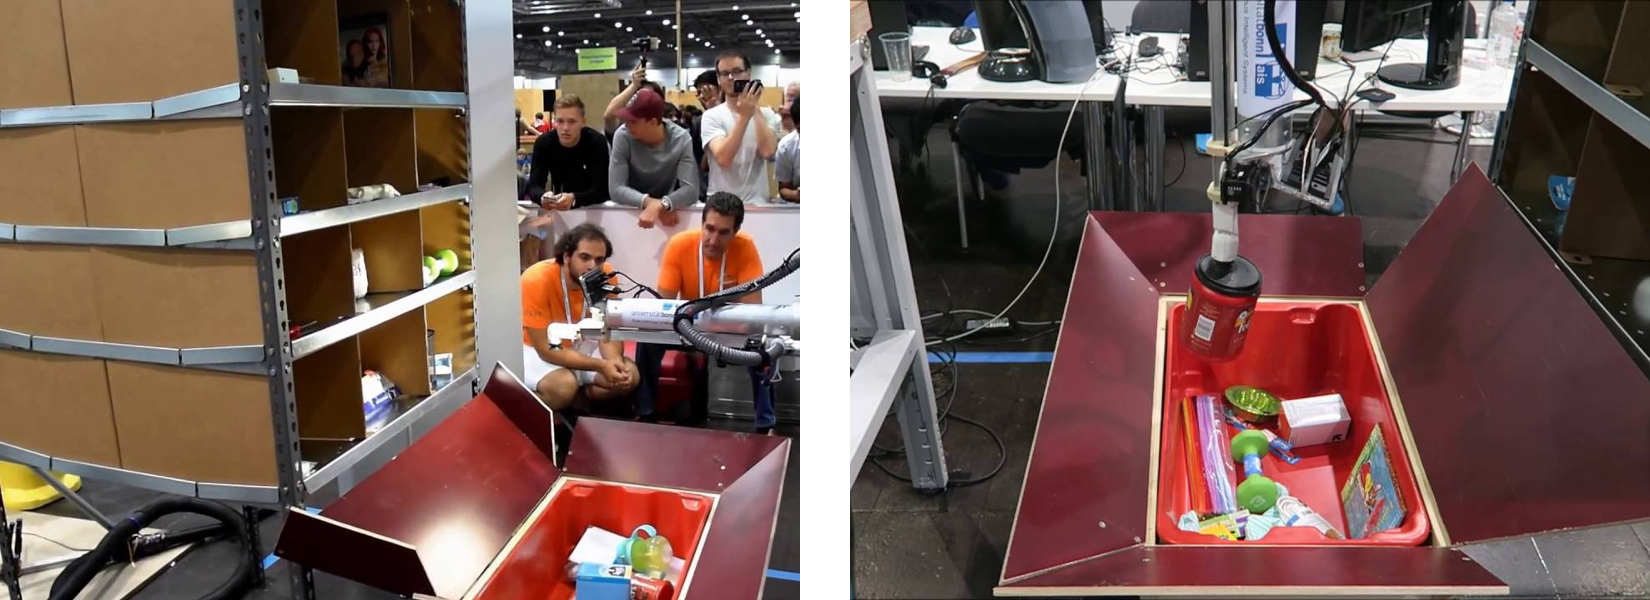
\includegraphics[width=0.8\textwidth]{figures/1_perception_and_sensing_in_robotics/amazon_picking_ch}
    \caption{\textbf{Amazon Picking Challenge example scenario.} In the images, the team is trying to detect and grasp objects from the red bin on the bottom, and place them on the shelf.} 
    \label{fig:amazon_picking_ch}
\end{figure}

The importance of robots in the industrial world is supported also by hi-tech giants, such as Amazon, Google and others, that in the last years demonstrated high interest in investing and developing their technologies in order to improve their performance and business. One interesting example is represented by the Amazon Picking Challenge competition proposed the first time at the International Conference on Intelligent Robots and Systems (IROS) in 2015 by the Amazon Robotics division\footnote{https://www.amazonrobotics.com}. This competition is thought to enhance and improve the research in the robotic manipulation, focusing the attention in grasping from random and highly cluttered environments, such as warehouse shelves or bins full of irregular and disorganized objects. In Figure \ref{fig:amazon_picking_ch}, some examples of typical tasks that teams involved in the Amazon Picking Challenge should compete.

\subsection{Random Bin Picking (RBP)}\label{subsec:binpicking}
Monotonous tasks such as unloading a bin one part at a time into a machine, bulk parts sorting, and order fulfillment are labor-intensive, moreover they can even be dangerous if the parts or operations are heavy, sharp and they change position every time one object is moved away. For years, bin picking robots have been tackling these tedious jobs, but there are still so many applications to be realized.

While more capable than ever, robotic bin picking still has its limitations. It is all matter of accuracy. While robots are applauded for their repeatability, random bin picking requires accuracy in the face of chaos. The robot has to locate a part in free space, in an unstructured environment where the parts keep shifting positions and orientations every time a part is removed from the bin. That requires a delicate balance between robotic dexterity, machine vision, software, computing power to crunch all the data in real time, and a grasping solution to extract the parts from the bin. All those highly technical challenges give to RBP higher complexity and difficulty.

First of all, a brief introduction to all the kinds of Bin Picking must be given. There are three main types of bin picking: structured, semi-structured, and random bin picking. Each presents an increasing level of application complexity, cost and cycle time:

\begin{itemize}
	\item \textbf{Structured}. Parts are positioned or stacked in the bin in an organized, predictable pattern, so they can be easily imaged and picked.
	\item \textbf{Semi-Structured}. Parts are positioned in the bin with some organization and predictability to help aid imaging and picking.
	\item \textbf{Random}. Parts are in totally random positions in a bin, including different orientations, overlapping, and even entangled, further complicating the imaging and picking functions.
\end{itemize}

From now on we will concentrate on Random Bin Picking, that is the main area in which we tested our work, moreover, the RAW dataset that will be presented later in this thesis and all the developed tools, have been thought for such robotic task in particular.

\begin{figure}
    \centering
    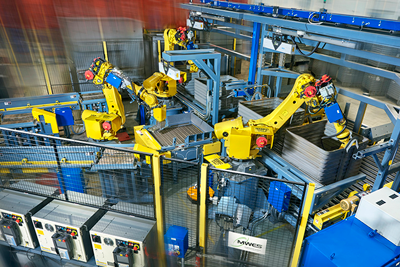
\includegraphics[width=0.8\textwidth]{figures/1_perception_and_sensing_in_robotics/rbp_example}
    \caption{\textbf{Random Bin Picking Example.} Robotic random bin picking and part loading system uses 3D vision guided robots with magnetic grippers to locate and pick parts for a heat treating operation.} 
    \label{fig:rbp_example}
\end{figure}

\begin{figure}
    \centering
    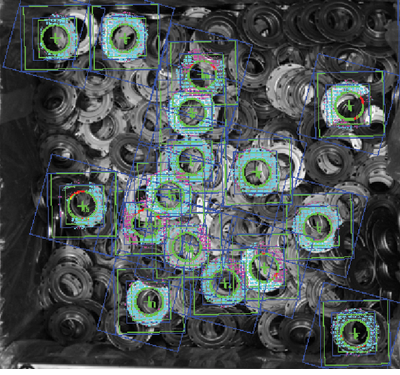
\includegraphics[width=0.5\textwidth]{figures/1_perception_and_sensing_in_robotics/cluttered_env_rbp}
    \caption{\textbf{Machine vision algorithm execution example in RBP task.} Here, a 3D area sensor is performing localization and recognition of random parts in a bin. Thanks to this technology, the robot should be capable of planning its next pick in the clutter.} 
    \label{fig:cluttered_env_rbp}
\end{figure}

An example of a robotic system performing random bin picking operation is depicted in Figure \ref{fig:rbp_example}. In this kind of scenarios, the role of vision is crucial. Vision systems must be capable of recognize, detect and localize the parts with extremely high accuracy. Typical scenarios are like the one in Figure \ref{fig:cluttered_env_rbp}, it's clearly visible how the environment is cluttered, all the parts are randomly spread inside the bin, and the task of recognizing and localizing the next part to be picked, it's extremely difficult. 

\subsection{Pick\&Place Tasks (PPT)}\label{subsec:pickandplace}
More generic, but with the same importance as the previous one, Pick\&Place (PPT) task is another interesting robotic application in which vision and perception play an important role. Differently from the aforementioned Bin Picking applications, in Pick\&Place scenarios, camera setup is not always fixed, they are mounted on the robotic arm, and the arm itself is not said to be fixed on the ground. 

A clear example of Pick\&Place scenario is the RoboCup@Work Competition, where the robotic arm that performs pick and drop operations with the objects, is actually mounted on a mobile platform that operates in a more large environment. Another example of robotic Pick\&Place operation are the robot assisted assembly \cite{evangelista2017grounding}, in which the robot assists the human in performing operation in industrial scenarios guided by natural language interaction.

\section{3D Scene Reconstruction}\label{sec:3dreconstruction}
In this section we are going to explore some techniques of 3D scene reconstruction for stereo cameras setup. This task has particular importance in the context of machine vision, since many object localization techniques are based on 3D approaches, so efficient methods for reconstructing the scene are needed. We will particularly focus on 3D stereo reconstruction approaches, since our experimental sensor setup is hardly based on this kind of technology, and we tested its performance with such algorithms and methods.

We will now address two techniques, namely \emph{Semi-Global Matching} from \cite{hirschmuller2005SemiGlobal} and\emph{PatchMatch Stereo} from \cite{bleyer2011PatchMatchStereo}. These two techniques have been intensively used as benchmark tools for our RAW dataset and our experimental sensor setup.

\subsection{Semi-Global Matching (SGM)}\label{subsec:semiglobalmatching}
Stereo matching is used to correlate points from one digital image of a stereo pair with the corresponding points in the second image of the pair. However, finding the best algorithms and parameters, is usually difficult, since different aspects must be considered: accuracy, completeness, occlusions, computational efforts, etc. The Semi-Global matching is, actually, one of the best matching strategies used both in photogrammetry and computer vision, offering good results with low runtime.

The Semi-Global Matching method from \cite{hirschmuller2005SemiGlobal} performs a pixel-wise matching allowing to shape efficiently object boundaries and fine details. 

The algorithm works with a pair of images, and their camera parameters, either intrinsic and extrinsic parameters must be known. That is because it assumes to know the epipolar constraint between the two images, the two cameras actually, so corresponding points are assumed to lie on the same horizontal image line, e.g. images have been rectified using such epipolar constraints. This algorithm realizes the minimization of a global smoothness constraint, combining matching costs along independent one-dimensional paths trough the image. The novel idea in SGM is that it actually computes the pixel matching cost through several paths in the image, not only on the horizontal epipolar line direction like it happened with previous implementations, e.g. scanline algorithm. All those paths and pixel-disparity pairs, aggregate in the computation of a cost function that SGM tries to minimize.

More in detail, the cost function $L^{\prime}_r(p, d)$ of the pixel $p$ and disparity $d$, along the path $r$ is defined as follow:

\begin{equation}\label{eq:sgm_cost_func}
    \begin{aligned}
    L^{\prime}_r(p, d) = &C(p, d) + 
    \min(L_r(p-r, d), \\
    &L_r(p-r, d-1)+P_1, \\
    &L_r(p-r, d+1)+P_2, \\
    &\min_iL_r(p-r,i)+P_2) - \min_kL_r(p-r,k)
    \end{aligned}
\end{equation}

In Eq. \ref{eq:sgm_cost_func} the first term $C(p, d)$ is the similarity cost (i.e. a value that penalizes, using appropriate metrics, solutions where different radiometric values are encountered in the neighbor area of the corresponding points), the second minimization term is for evaluating the regularity of the disparity field, in fact there are two penalization terms $P_1$ and $P_2$ that basically control small and large change in the disparity with respect to the previous point along the matching path $r$. In the end there is a regularization term that allows to reduce the final value subtracting the minimum path cost of the previous pixel from the amount, if no regularization term is used, the cost tends to gradually increase during cost aggregation along the path.

Minimizing such cost function for a 2D image space is a NP-complete problem. SGM minimizes the cost by means of Dynamic Programming, with the novel idea of computing the optimization combining several individual path, symmetrically from all directions through the image. Summing the path costs in all directions and searching the disparity with the minimal cost for each image pixel $p$, produces the final disparity map.

\subsection{PatchMatch Stereo}\label{subsec:patchmatchstereo}
To do ...

\section{Object Detection}\label{sec:objectdetection}
In the following sections we will introduce some machine vision algorithms and techniques for object detection. In particular it will be shown a comparison between standard state of the art techniques based on shape-based approaches, and deep learning networks oriented to object detection and recognition.

\subsection{D\textsuperscript{2}{CO} Algorithm}\label{subsec:d2co}
As already anticipated, standard approaches are based on object shape and appearance. This means that a CAD model of the object is needed, since the algorithm mainly works on edges extraction and some sort of template matching between the projected model and the edges extracted from the image.

An example of standard algorithm that is totally based on shape and edges is the one presented in \cite{imperoli2015d2co}. This is the very same approach used also in RoboCup@Work by the SPQR@Work team for performing the final registration step in the object detection pipeline. 

\begin{figure}
    \centering
    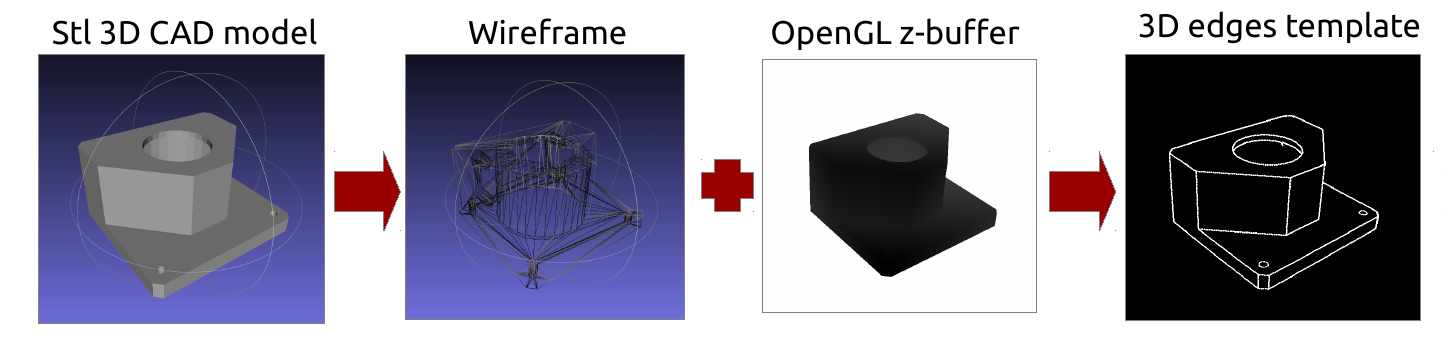
\includegraphics[width=\textwidth]{figures/1_perception_and_sensing_in_robotics/d2co_00}
    \caption{\textbf{D\textsuperscript{2}CO input data example}. The raster models used in D\textsuperscript{2}CO are computed from the 3D CAD models of the objects.} 
    \label{fig:d2co_00}
\end{figure}

The algorithm is called D\textsuperscript{2}{CO}, namely Direct Directional Chamfer Optimization. D\textsuperscript{2}CO refines the object position employing a non-linear optimization procedure, where the cost being minimized is extracted directly from a 3D image tensor composed by a sequence of distance maps. No ICP-like iterative re-association steps are required: the data association is implicitly optimized while inferring the object pose. This approach is able to handle textureless and partially occluded objects and does not require any off-line object learning step: just a 3D CAD model is needed (see Figure \ref{fig:d2co_00}).

The Directional Chamfer Distance (DCD) tensor encodes the minimum distance of an image point to an edge point in a joint direction/location space. Unlike the Chamfer distance, the DCD takes into account also the edges directions, see Figure \ref{fig:d2co_01} for further explanations.

The algorithm extract a set of object candidates by pre-computing the (projected) raster templates along with their image orientations for a large number of possible 3D locations; for each point, it looks up the DCD tensor, computing the template average distance. The templates are then sorted for increasing distances. D\textsuperscript{2}CO finally refines the object position employing a non-linear optimization procedure that minimizes a tensor-based cost function, look at Figure \ref{fig:d2co_02} for a registration example. Then, the Levenberg Marquardt algorithm with a Huber loss function is used in order to reduces the influence of outliers. During the optimization, both the (projected) points position and the (projected) points orientation are constantly updated.

\begin{figure}
    \centering
    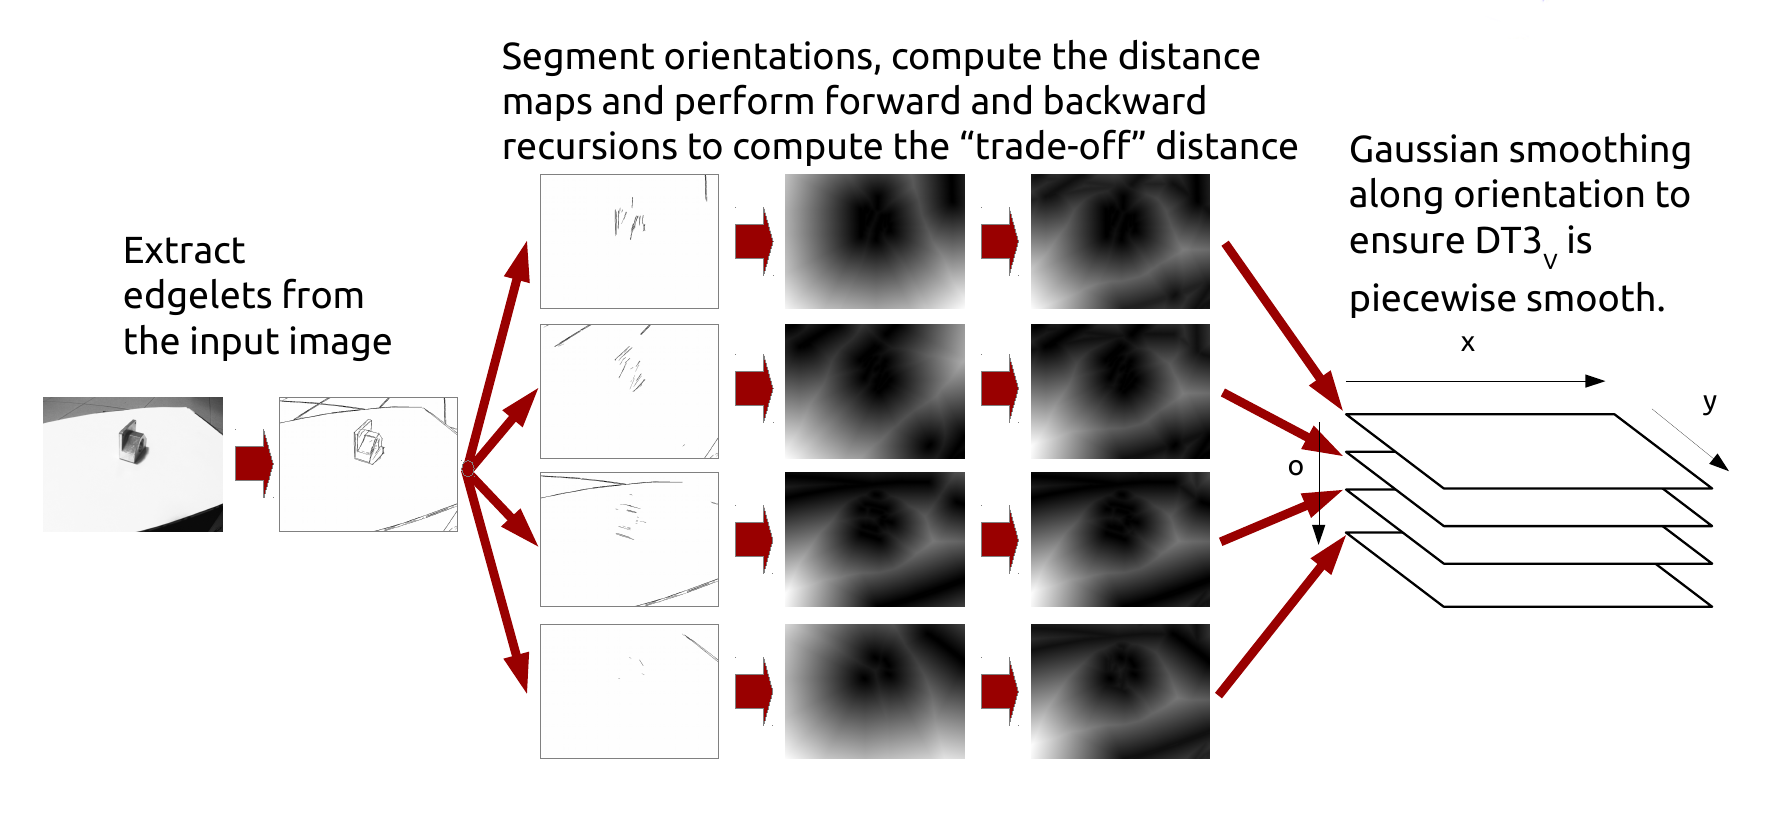
\includegraphics[width=\textwidth]{figures/1_perception_and_sensing_in_robotics/d2co_01}
    \caption{\textbf{Directional Chamfer Distance}. DCD tensor computation pipeline.} 
    \label{fig:d2co_01}
\end{figure}

\begin{figure}
    \centering
    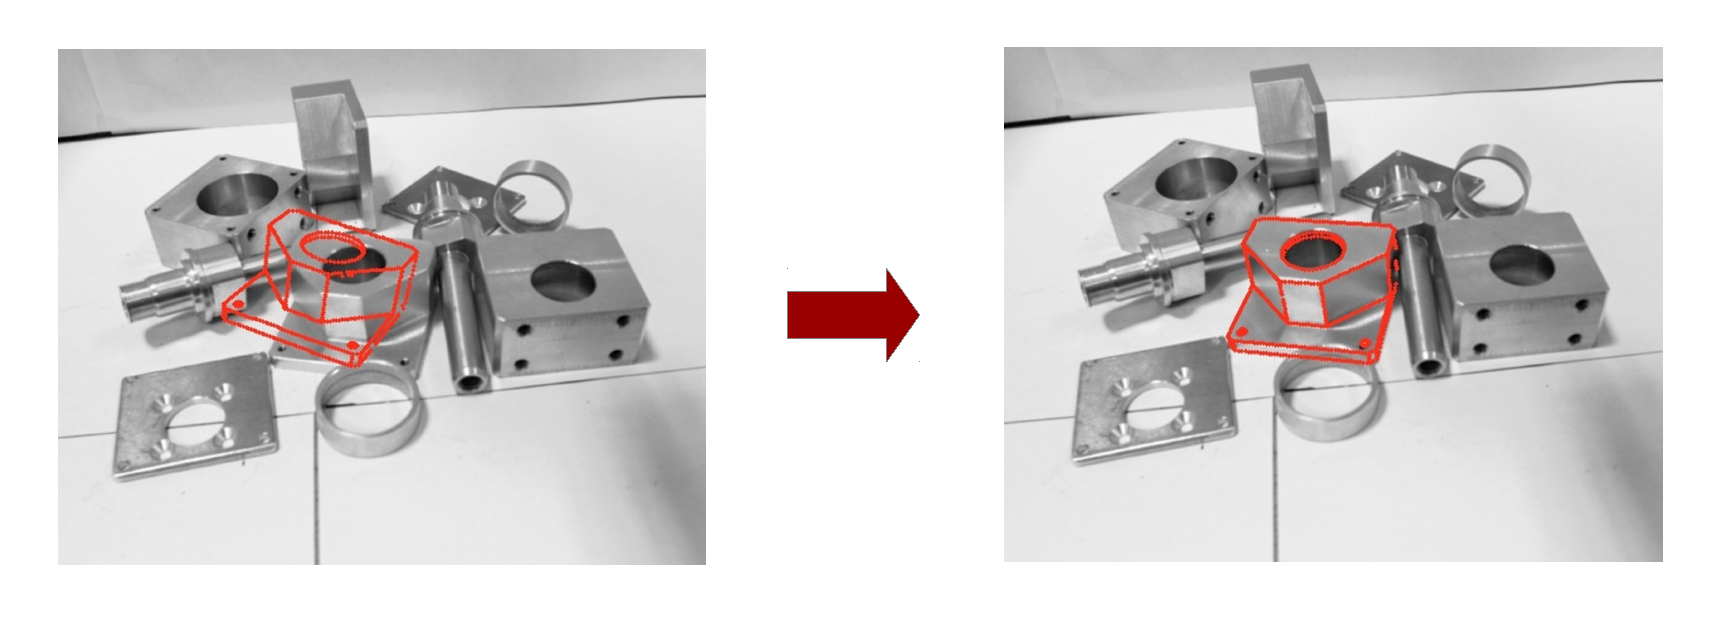
\includegraphics[width=\textwidth]{figures/1_perception_and_sensing_in_robotics/d2co_02}
    \caption{\textbf{D\textsuperscript{2}{CO} Registration Example}. An example of object registration using the D\textsuperscript{2}{CO} algorithm.} 
    \label{fig:d2co_02}
\end{figure}

\subsection{Deep Learning Neural Networks for Object Detection}\label{subsec:dl_obj_detection}
Despite standard techniques for object detection like the one introduced in the last section, here we are going to explore some techniques that in the recent years have become the state of the art in most of the common computer vision tasks, such as object detection. Those approaches are based on \emph{CNNs (Convolutional Neural Networks)} and are commonly associated with the Deep Learning literature. In Machine Learning in fact, CNN is a class of deep, feed-forward artificial neural network. 

The idea of this kind of networks comes from biological processes: 

\begin{itemize}
	\item The connectivity pattern between neurons is inspired by the organization of the animal visual cortex; 	
	\item Individual cortical neurons respond to stimuli only in a restricted region of the visual field known as the receptive field; 
	\item The receptive fields of different neurons partially overlap such that they cover the entire visual field.
\end{itemize}

Following those intuitions, also in Computer Vision, more in detail in image processing, CNNs have been applied analyze and process visual data such as our brain does. CNNs use relatively little pre-processing compared to other image classification algorithms. This means that the network learns the filters that in traditional algorithms were hand-engineered. This independence from prior knowledge and human effort in feature design is a major advantage and is something that comes directly from the input data used during the training phase of the network, that is why this kind of approaches are also called \emph{data driven}, because they mostly relies on huge amounts of data.

More in detail a CNN consists of an input and an output layer, as well as multiple hidden layers. Those hidden layers typically consist of convolutional layers, pooling layers, fully connected layers and normalization layers. In particular:

\begin{itemize}
	\item \textbf{Convolutional Layer}: Convolutional layers apply a convolution operation to the input, passing the result to the next layer. The convolution emulates the response of an individual neuron to visual stimuli. Each neuron here processes data only for its receptive field. Those kind of input partitioning allows CNNs to tolerate translation of the input image (e.g. translation, rotation, perspective distortion, etc.)
	\item \textbf{Pooling Layer}: Those kind of layers combine the outputs of neuron clusters at one layer into a single neuron in the next layer. For example, max pooling uses the maximum value from each of a cluster of neurons at the prior layer. Pooling layers are commonly used after convolutional ones in order to reduce the dimension of the data, also called data dimensionality reduction.
	\item \textbf{Fully Connected Layer}: Fully connected layers connect every neuron in one layer to every neuron in another layer. It is in principle the same as the traditional multi-layer perceptron neural network (MLP).
\end{itemize}

\begin{figure}
    \centering
    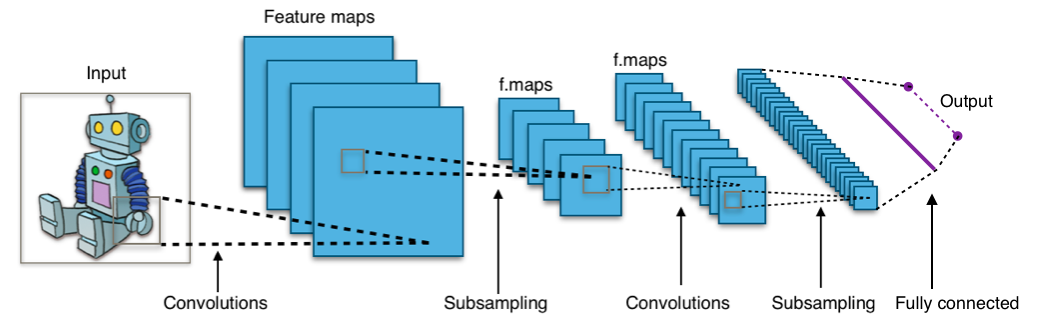
\includegraphics[width=\textwidth]{figures/1_perception_and_sensing_in_robotics/typical_cnn}
    \caption{\textbf{Typical CNN architecture}. Typical CNNs architectures are composed by single or many convolutional layers, each followed by some pooling layer in order to reduce the dimension of the data for the next convolutional layer. As our scope is to evaluate object detection and classification results, commonly used architectures uses fully connected layer at the end of the network for performing classification.} 
    \label{fig:typical_cnn}
\end{figure}

An example of a typical CNN architecture is given in Figure \ref{fig:typical_cnn}.

\section{State of the art Software Libraries in Industry}\label{sec:industrylibraries}
Machine Vision is one of the most active area in industrial settings. Over the past years, many software companies and Open Source communities have dedicated lot of effort in developing robust and effective techniques and algorithms in order to assist industrial realities, such as companies and start ups, in performing computer vision assisted tasks, e.g. random bin picking, Pick\&Place tasks and so on.

In the following subsection a list of tools and libraries will be introduced, focusing mainly on the MVTec's Halcon Libraries, which are the one that we used in the experiment phase of this work. 

\subsection{Halcon Libraries}\label{subsec:halconlibs}
Halcon\footnote{http://www.mvtec.com/products/halcon/}, from MVTec, is a set of commercial software developed and sold explicitly for industrial settings. Over the past 5 years it has become the state of the art in machine vision for industrial tasks. It serves all industries with an extensive library of more than 1600 operators for blob analysis, morphology, matching, measuring, identification, and 3D vision, to name just a few.

The full library can be accessed from common programming languages like C, C++, C\#, Visual Basic .NET, and Delphi. In particular, our tests have been developed using the C++ APIs. In the following chapters we will test this standard Machine Vision approaches over the RAW and T-Less datasets, and compare them with completely different approaches such as Deep Learning CNNs for object localization and recognition.

\begin{figure}
    \centering
    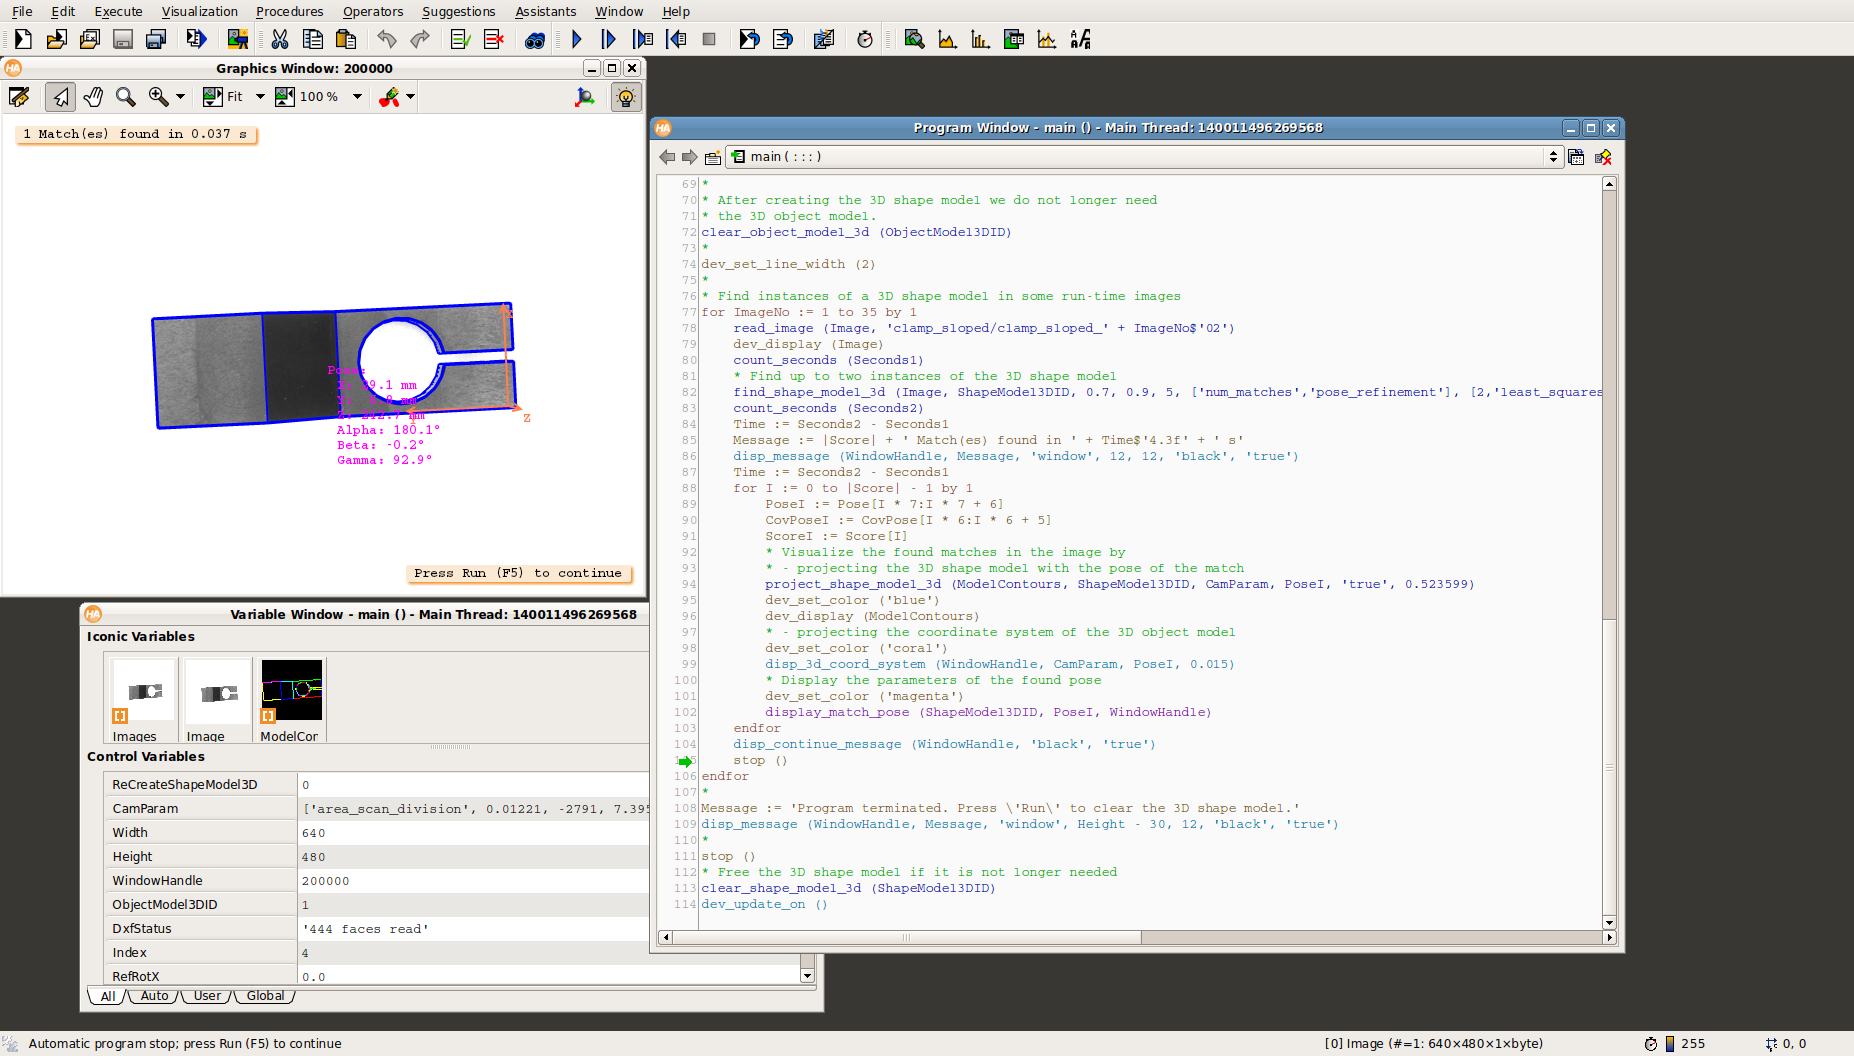
\includegraphics[width=0.8\textwidth]{figures/1_perception_and_sensing_in_robotics/hdevelop_gui_example}
    \caption{\textbf{Hdevelop GUI example.} An example of using the Hdevelop software from the Halcon Libraries. In particular here we are performing an object detection and localization task.} 
    \label{fig:hdevelop_example}
\end{figure}

The Halcon Library has also an interactive and friendly GUI, provided in order to facilitate the interfacing with the low level software APIs. The aforementioned software tool is called HDevelop, and an example of its usage and graphical interface is depicted in Figure \ref{fig:hdevelop_example}.

As anticipated, this software library is under commercial license, and our distribution has been sold to La Sapienza University of Rome that can use it for research and other non-commercial purposes. 

\begin{figure}
    \centering
    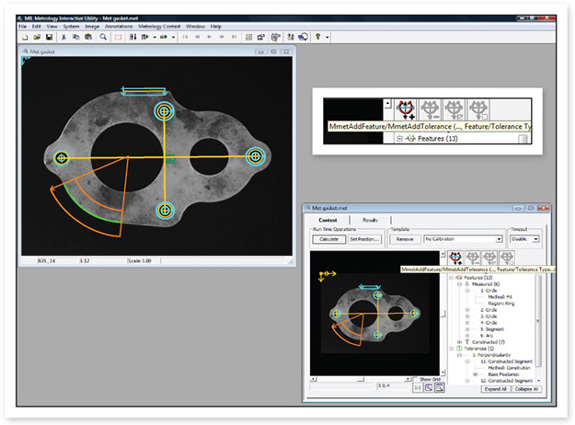
\includegraphics[width=0.8\textwidth]{figures/1_perception_and_sensing_in_robotics/mil_gui_example}
    \caption{\textbf{MIL GUI example.} The graphical user interface of the Matrox Imaging Library.} 
    \label{fig:mil_example}
\end{figure}

\subsection{Matrox Imaging Library (MIL)}\label{subsec:mil}
Another important software library that needs to be mentioned is the Matrox Imaging Library\footnote{https://www.matrox.com/imaging/en/products/software/mil/} (MIL). MIL is a complete collection of software tools for developing machine vision in lots of different scenarios, it is not restricted to the industrial one such as for the previously mentioned Halcon Libraries, but it covers also medical images applications and many others.

MIL includes also a graphic user interface for fast developing and prototyping of solutions. An example of this GUI is depicted in Figure \ref{fig:mil_example}.

This library is not part of the tests and examples performed during this work.